\chapter{Literature Review}
Currently state of the art models in machine learning often perform best when using a pretrained backbone which is often trained on well known public datasets, such as ImageNet \cite{deng2009imagenet} for image related tasks or Common Crawl \cite{commoncrawl} for text-based tasks. These pretrained backbones or foundation models, are then used for fine-tuning on specific tasks.

The main benefit of using pretrained networks are two-fold: they typically improve the convergence speed of the model and reduce the amount of task-specific data required \cite{donahue2014decaf,zeiler2014visualizing}. Furthermore, many the state of the art models in various (image) related task, such as object detection\cite{liu2016ssd,redmon2016you} and semantic segmentation \cite{orsic2019defense,girshick2014rich} benefit from pretrained backbones.

A drawback of these generic datasets is that, in many real-world robotic applications, the actual data distribution encountered is a tiny subset of those seen during training. E.g. a robot tasked with navigating in an indoor warehouse is unlikely to encounter an elephant. Thus the parts of the pretrained model that are able to detect elephants, or other animals, will not be used and take up precious computational resources on the device. Thus by pretraining a model on the actual data distribution it will encounter, the model could be made smaller or achieve higher accuracy.

However, the downside is that current pretraining tasks usually require the data to be labeled, which is an expensive endevor. Therefor, having a unsupervised pretraining method could be beneficial. A Variational Auto-Encoder (VAE) can be trained purely on images without requiring any manual labeling.

\section{VAE}
The VAE was first proposed by Kingma et al. \cite{kingma2014autoencodingvariationalbayes}. The task of a VAE is to reconstruct an image based on a (smaller) latent variable, and thus results in a type of lossy compression. The objective function of an VAE is the evidence lower bound (ELBO) \ref{eq:elbo}.
\begin{equation}
    \label{eq:elbo}
    \mathcal{L} = \mathbb{E}_{q_{\phi}(z|x)}[\log p(x|z)] - D_{KL}(q_{\phi}(z|x) || p(z))
\end{equation}
where $\mathcal{L}$ is the ELBO, $x$ represents the input data, $z$ is the latent variable, $p(x|z)$ is the likelihood of observing the input data given the latent variable, $q_\phi(z|x)$ is the variational distribution or approximate posterior, and $D_{KL}(q_{\phi}(z|x) || p(z))$ is the Kullback-Leibler (KL) divergence between the variational distribution and the prior. By choosing a prior for which the KL divergence can be integrated analytically, we only need to approximate the reconstruction error $\mathbb{E}_{q_{\phi}(z|x)}[\log p(x|z)]$ using sampling. This allows us to efficiently optimize the VAE's parameters and reduce the computational complexity of training. Moreover, the learned latent representation of the VAE can be used as a pre-training method for training an encoder, which can then be fine-tuned for specific image segmentation tasks.

The distributions $q_{\phi}(z | x)$ and $p_{\theta}(x | z)$ can be approximated using neural networks. To allow the model can be optimized using stochastic gradient descent, the reparameterization trick is used.

One problem with VAEs is that their latent representation are not typically 'disentangeld'. Meaning, that one latent unit is sensitive to a single factor of the generative properties of the data. For instance, when generating human faces, a single latent value should only influence the age, not other features such as the shape of the nose or eyes. When the latent variables are properly disentangeld, they can provide a good representation which can be used by other models on subsequent task \cite{bengio2014representationlearningreviewnew}. The $\beta$-VAE, proposed by Higgins et al. \cite{higgins2017betavae}, multiplies the KL divergence with a hyperparameter $\beta$. If this value is set to 1, it results in a standard VAE. In their paper, they show that for $\beta$ values greater then one, the learnt latent representation are more disentangeld. Note, that there is no additional information required about the data for this to be learned. By increasing the $\beta$, the capacity of the latent space is reduced. Meaning, that less information can be passed due to the stronger regularization force of the KL-divergence.

Top-Down Hierarchical VAEs \cite{maaloe2019biva,NIPS2016_6ae07dcb,vahdat2020nvae} are a further improvement, which mainly tackle the sharpness and coherency of the generated images. These models consist of multiple latent spaces, each learned from different depths within the encoder.

\subsection{Anomaly Detection}
Due to the probabilistic nature of the VAE, it can also be used for anomaly detection. There are two main methods with which this can be done. Either from the posterior output $p_{\phi}(z|x)$, by detecting unusual latent variables \cite{marimont2020anomalydetectionlatentspace,angiulli2020improving,angiulli2023latent}. Or calculating the reconstruction error from the given input \cite{an2015variational, zhou2020unsupervisedanomalylocalizationusing, gouda2022unsupervised}. The main benefit of the first method is that the decoder is not required for anomaly detection, resulting in a lower inference cost. In the case of robotics, it is important to detect unusual situation as it might result in unexpected behaviour which inturn could lead to dangerous situations.
A closely related use case is the ability to have an uncertainty estimation, by the use of bootstrapping \cite{chen2018use,kohl2018probabilistic}, for the output of the model. The additional uncertainty information could then be used by downstream systems to be even more robust. Furthermore, this information can be used for various active learning \cite{hino2020active} techniques. Which allow for more effective labeling strategies, thus reducing the amount of labeling required.

\section{Semantic Slam}
Simultaneous localication and mapping (SLAM)\cite{chatila1985position} is a powerful method used for the automated navigation of robotic vehicles. It is capable of simultaneously creating a map of an unknown environment and navigating that same environment. A vital part for autonomous robotic vehicles. With the rise of deep learning methods in computer vision, many visual based SLAM algorithms have been created \cite{taketomi2017visual}. More recent algorithms use semantic segmentation networks \cite{yu2018ds}. It uses SegNet \cite{badri2017segnet}, to extract the semantic information from images. By improving the quality of this model, the complete system would become more stable.

\subsection{Semantic segmentation}
Semantic segmentation is a computer vision technique that involves assigning a label or category to each pixel in an image. This means that, rather than just detecting objects, the method also identifies what those objects are (e.g., chair, person, road). The goal of semantic segmentation is to produce a dense prediction map that classifies every pixel in the image into one of the predefined categories.

One of the first more successful deeplearning methods for semantic segmentation was the Fully Convolutional Network (FCN) proposed by Long et al. \cite{long2015fully}. Which was slightly improved by \cite{ronneberger2015u}, and named U-net. Referencing the shape of the model. The architecture of the model can be seen in Figure \ref{fig:unet-architecture}. Due to the structure, the output can take both fine-grained information, which is useful to have good localization and global information, which improves the classification. This method is robust and reliable, making it easy to train and use in real-time applications.
\begin{figure}[ht]
    \centering
    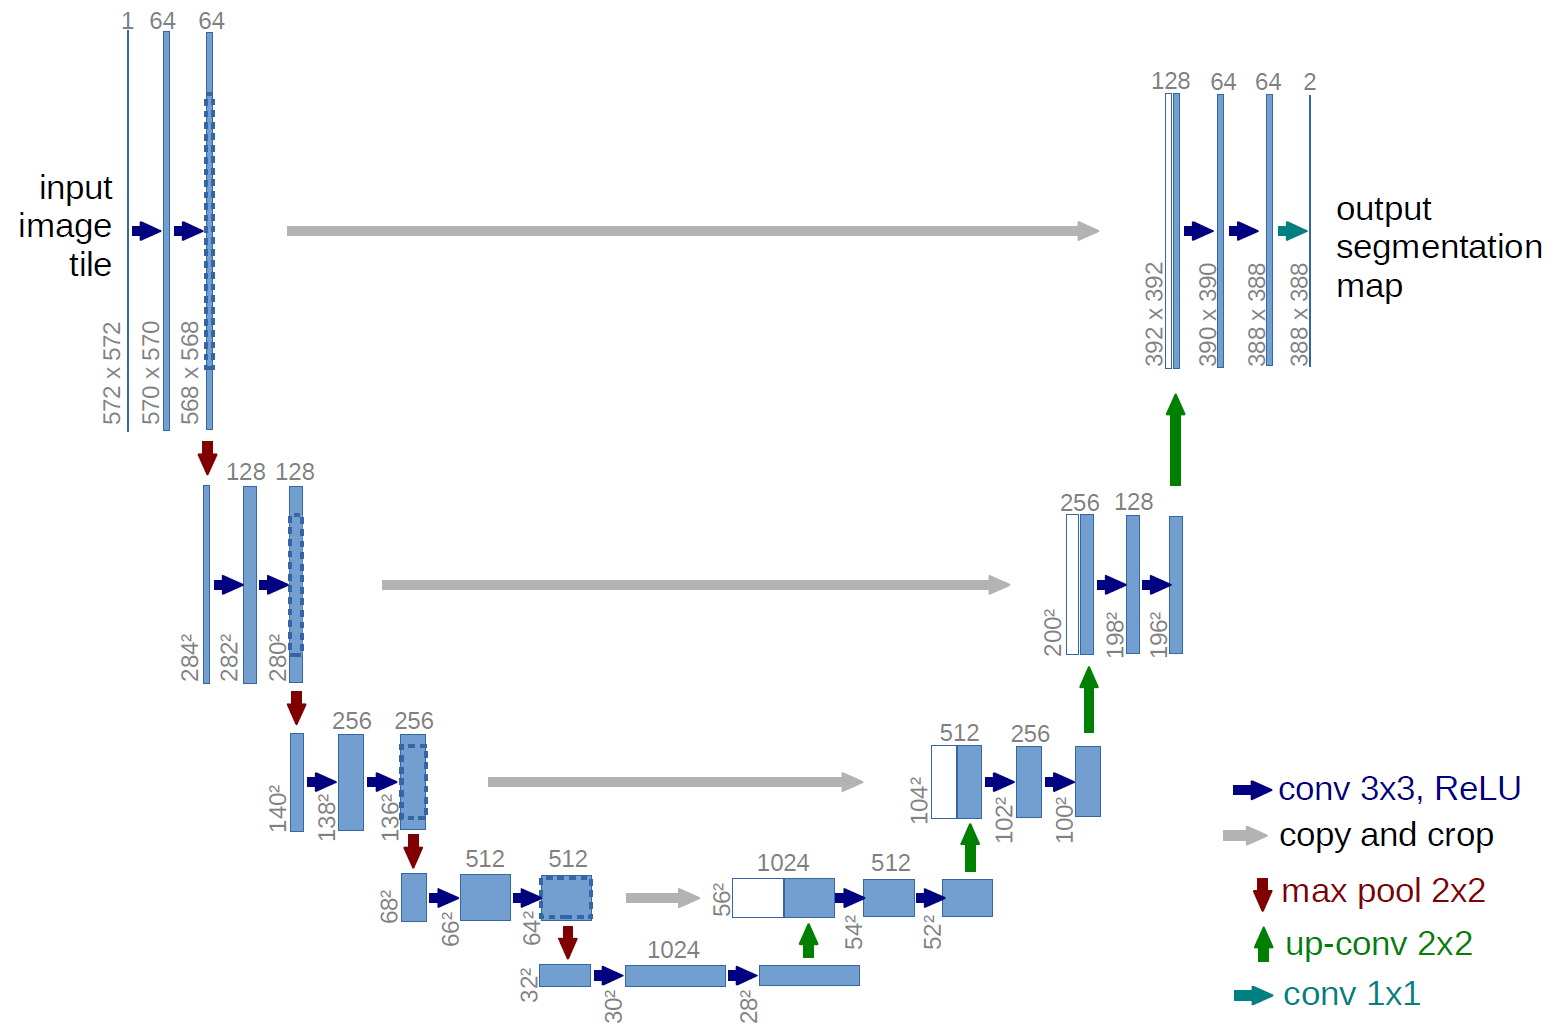
\includegraphics[width=0.5\textwidth]{figures/unet-architecture.png}
    \caption{U-Net Architecture \cite{ronneberger2015u}}
    \label{fig:unet-architecture}
\end{figure}

Feature Pyramid Network (FPN) \cite{lin2017feature} shares part of it structure with the UNet. Except it explicitly combines the features of each upscaling layer to predict the final semantic segmentation mask as visualized in Figure \ref{fig:fpn-architecture}. The main difference between FPN and U-Net is that FPN takes more time to process images. It does produce better results for smaller and medium-sized objects.

\begin{figure}[ht]
    \centering
    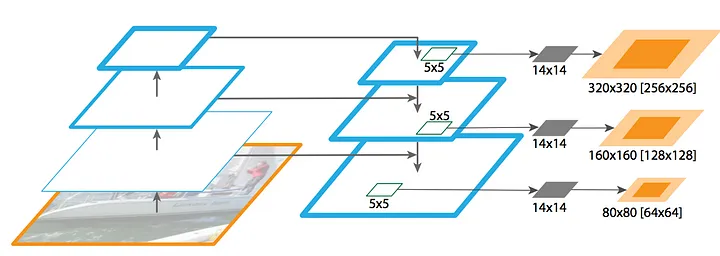
\includegraphics[width=0.5\textwidth]{figures/fpn-architecture.png}
    \caption{Feature Pyramid Network Architecture \cite{lin2017feature}}
    \label{fig:fpn-architecture}
\end{figure}

Although the above models are not state of the art anymore, they remain easy to train and do not require exotic tricks to make them work. Moreover, they have good inference speed and are architecturely similar to our proposed method. The primary issue with these models is their limited field of view, resulting in dificulty in relating parts of the image that are far apart. This can partially be combated by making use of dilated convolutional layers, such as proposed by Gao \cite{gao2023rethinking}. Or by the use of vision tranformers \cite{dosovitskiy2021image}, which can relate pixels that are far apart in the input image. These vision tranformers have been used successfully in the segmentation task \cite{xie2021segformer,chen2022vision}. However, due to the computational complexity in vision tranformers they are not yet suitable for real-time inference on mobile robotics.

Another impressive example is the Segment Anything Model (SAM) \cite{kirillov2023segment}. It is a huge, and slow, network capable of, as the name implies, anything based on a prompt. Although not relevant for comparison, it can be used to aid the labour intensive task of labeling new data.
